\documentclass[11pt]{article}
\usepackage[utf8]{inputenc}	% Para caracteres en español
\usepackage{amsmath,amsthm,amsfonts,amssymb,amscd}
\usepackage{multirow,booktabs}
\usepackage[table]{xcolor}
\usepackage{fullpage}
\usepackage{lastpage}
\usepackage{enumitem}
\usepackage{fancyhdr}
\usepackage{mathrsfs}
\usepackage{wrapfig}
\usepackage{setspace}
\usepackage{calc}
\usepackage{multicol}
\usepackage{cancel}
\usepackage{float}
\usepackage{physics}
\usepackage[retainorgcmds]{IEEEtrantools}
\usepackage[margin=1cm]{geometry}
\usepackage{amsmath}
\newlength{\tabcont}
\setlength{\parindent}{0.0in}
\setlength{\parskip}{0.05in}
\setlength{\headheight}{14pt}
\usepackage{empheq}
\usepackage{framed}
\usepackage[most]{tcolorbox}
\usepackage{xcolor}
\usepackage[version=3]{mhchem}
\usepackage[english]{babel}
\usepackage[utf8]{inputenc}
\usepackage{graphicx}
\usepackage[colorinlistoftodos]{todonotes}
\usepackage{mdframed}

\colorlet{shadecolor}{orange!15}
\parindent 0in
\parskip 12pt
\geometry{margin=1in, headsep=0.25in}
\theoremstyle{definition}
\newtheorem{defn}{Definition}
\newtheorem{reg}{Rule}
\newtheorem{exer}{Exercise}
\newtheorem{note}{Note}
\numberwithin{equation}{section}
\begin{document}
%\setcounter{section}{2}
%\setcounter{subsection}{}
\title{Finals}

%==============================================================
%\thispagestyle{empty}
\pagestyle{fancy}
\fancyhf{}
\rhead{Physics 180}
\chead{Finals}
\lhead{Olyn D. Desabelle}
\rfoot{Page \thepage}

\begin{center}
{\LARGE \bf Finals}\\
%{\large Physics 180}\\
%Olyn D. Desabelle
\end{center}

\begin{mdframed}
    I swear upon my honor that I have not given nor received any unauthorized help on this exam and that all the work below are my own.
\end{mdframed}
\begin{figure}[H]
    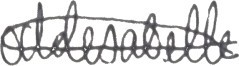
\includegraphics[scale = 20]{my e-sig.jpg}
\end{figure}

DESABELLE, Olyn D.

\noindent\makebox[\linewidth]{\rule{\paperwidth}{0.4pt}}

\section{\textbf{Baa Baa Black Sheep} [50 pts.]}

%Bhabha scattering
%https://www.pas.rochester.edu/assets/pdf/undergraduate/Example_of_Lowest-Order_Processes_in_QED.pdf
%https://www.hep.phy.cam.ac.uk/~thomson/partIIIparticles/handouts/Handout_4_2011.pdf

\begin{figure}[H]
    \centering
    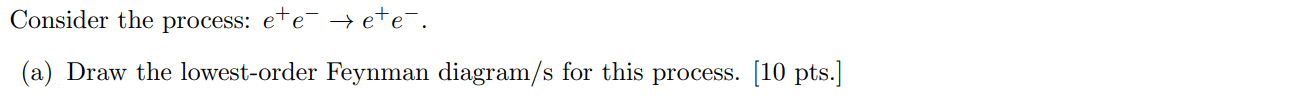
\includegraphics[scale = 0.4]{1a.png}
\end{figure}

There are two lowest-order Feynamn diagrams for this process. One is the pair annihilation represented by an s-channel diagram:

[insert here]

and the other is the scattering represented by a t-channel diagram:

[insert here]

%\begin{align} Z =
%\begin{cases}
%    \frac{-a_v  A^2 + a_s A^{5/3} - a_c A^{2/3} -A + a_p A^{1/2}}{-[2 - 2 (a_c A^{2/3})]}& \text{ for even } A,\text{ odd Z}\\
%    \frac{-a_v  A^2 + a_s A^{5/3} - a_c A^{2/3} -A - a_p A^{1/2}}{-[2 - 2 (a_c A^{2/3})]}& \text{ for even } A,\text{ even Z}\\
%    \frac{-a_v  A^2 + a_s A^{5/3} - a_c A^{2/3} -A}{-[2 - 2 (a_c A^{2/3})]}& \text{ for odd } A
%\end{cases}
%\end{align}


%==============================================================
\newpage
%==============================================================



\begin{figure}[H]
    \centering
    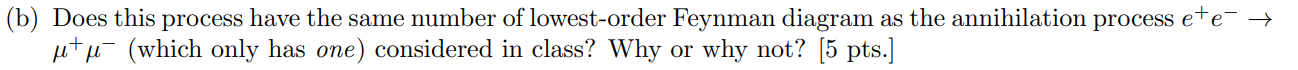
\includegraphics[scale = 0.4]{1b.png}
\end{figure}

The process $e^+e^- \to e^+e^-$ does not have the same number of lowest-order Feynman diagram as the $e^+e^- \to \mu^+\mu^-$ process since the former has 2 while the latter only has 1. This is because


%==============================================================
\newpage
%==============================================================



\begin{figure}[H]
    \centering
    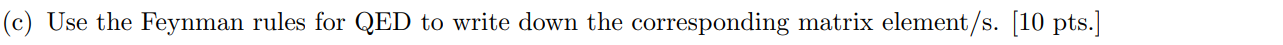
\includegraphics[scale = 0.4]{1c.png}
\end{figure}

\underline{s-channel annihilation}

Lorem

\underline{t-channel scattering}


%==============================================================
\newpage
%==============================================================


\begin{figure}[H]
    \centering
    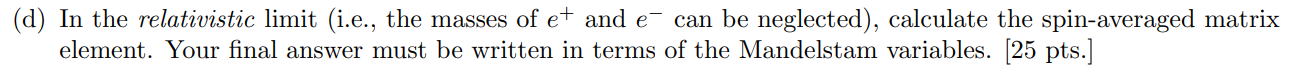
\includegraphics[scale = 0.4]{1d.png}
\end{figure}


%==============================================================
\newpage
%==============================================================

%==============================================================
%we then note that we can switch up the order of differentiation:

\section{\textbf{Look At Me Roll} [50 pts.]}
%============================================================

%Moller scattering

\begin{figure}[H]
    \centering
    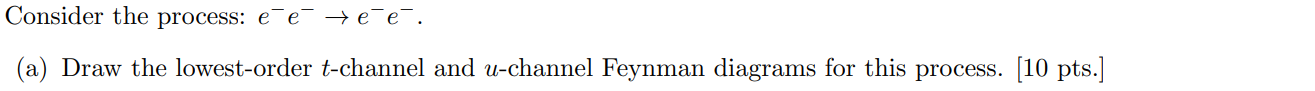
\includegraphics[scale = 0.4]{2a.png}
\end{figure}

The lowest-order t-channel Feynman diagram for the process is given by:

[insert here]

The lowest-order u-channel Feynman diagram for the process is given by:

[insert here]

%==============================================================
\newpage
%==============================================================



\begin{figure}[H]
    \centering
    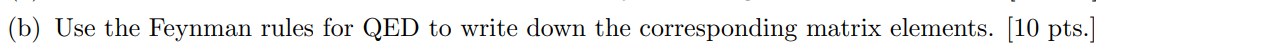
\includegraphics[scale = 0.4]{2b.png}
\end{figure}

We note that the Feynman rules for QED note the following contributions to the matrix element $\mathcal{M}$

\underline{t-channel}

For the t-channel Feynman diagram, the matrix element $\mathcal{M}$ is given by:

\underline{u-channel}

For the u-channel Feynman diagram, the matrix element $\mathcal{M}$ is given by:
%==============================================================
\newpage
%==============================================================


\begin{figure}[H]
    \centering
    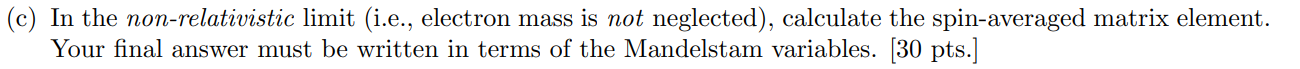
\includegraphics[scale = 0.4]{2c.png}
\end{figure}

We note that the spin-averaged matrix element is given by:

\underline{t-channel}

For the t-channel Feynman diagram, 

\underline{u-channel}

For the u-channel Feynman diagram,
%==================================
%helpful ps8 and ps9
\end{document}